\documentclass[12pt]{article}
\usepackage[a4paper]{geometry}
\usepackage[pdftex]{hyperref}
\usepackage[german]{babel}
\usepackage[utf8]{inputenc}
\usepackage{csquotes}
\usepackage{amssymb}
\usepackage{graphicx}
\usepackage{multicol}
\usepackage{amsmath}
\usepackage{enumitem}
\usepackage{tabularx}
\usepackage{vwcol}
\usepackage{fancyhdr}
\usepackage{indentfirst}
\usepackage{polynom}

\geometry{
  headheight=14px,
  left=2.54cm,
  right=2.54cm,
  bottom=2cm,
  top=2cm
}

% For horizontally centering text in Y column
\newcolumntype{Y}{>{\centering\arraybackslash}X}

\setlength{\parindent}{0cm}

\setlength{\marginparsep}{1 cm}
\setlength{\topmargin}{-0.6in}
\setlength{\textheight}{9.5in}
\pagestyle{fancy}

% German-style quotation marks %
\MakeOuterQuote{"}

% Typesetting differential operator %
\providecommand\d{}
\renewcommand{\d}[1]{\:\mathrm{d}{#1}} 

% For vertical centering text in X/Y column
\renewcommand\tabularxcolumn[1]{m{#1}}

\polyset{%
   style=C,
   delims={\big(}{\big)},
   div=:
}

\fancypagestyle{firstpage}{%
  \lhead{\bf Staatliche Studienakademie Dresden\\
Studienrichtung: Informationstechnologie}
  \rhead{\bf Datum: 13.02.2019}
}

\cfoot{\thepage\ of \pageref*{LastTask}}

\begin{document}

\thispagestyle{firstpage}

\begin{flushright}
Anzahl der Klausurblätter: \pageref*{LastTask}
\end{flushright}

Probeklausur im Lehrgebiet: Algebra/Analysis\\

Teilgebiet: Analysis \\

Modulcode: 3MI-MATHE-10 \\

Lehrender: Andre Wachsmuth \\

Semester: 1 \\

\begin{vwcol}[widths={0.4,0.4,0.2},sep=0cm, justify=flush,rule=0pt,indent=4em]
Name:\\
Vorname:\\
SG:
\end{vwcol}

\bigskip
\bigskip
\bigskip
Bearbeitungszeit: 40 min \\

Zugelassene Hilfsmittel: 1 handbeschriebenes A4-Blatt \\

\textbf{Es dürfen keine eigenen Zusatzblätter abgegeben werden.} \\

\textbf{Verwenden Sie auch die Blattrückseiten für Antworten! Markieren Sie deutlich, zu welcher Frage die auf Rückseiten gegebenen Antworten gehören.} \\

\textbf {Der Rechengang muss eindeutig und vollständig ersichtlich sein!} \\

Punkteverteilung:

\bigskip

\begin{tabularx}{\textwidth}{l|Y|Y|Y|Y|Y|Y}
Aufgabe        & 1 & 2 & 3 & 4  & Zusatz & Summe \\ [1ex] \hline
Soll-Punktzahl & 7 & 7 & 8 & 8  & 2      &       \\ [3ex]
Ist-Punktzahl  &   &   &   &    &        &       \\ [3ex]
\end{tabularx}

\newpage
\section* {Aufgabe 1}

In der folgenden Skizze ist die Funktion $f(x)=\frac{x}{\sin(x)}$ dargestellt. Weiterhin ist die Funktion $g(x)$ dargestellt, welche aus $f$ durch Verschiebung hervorging.

\begin{center}
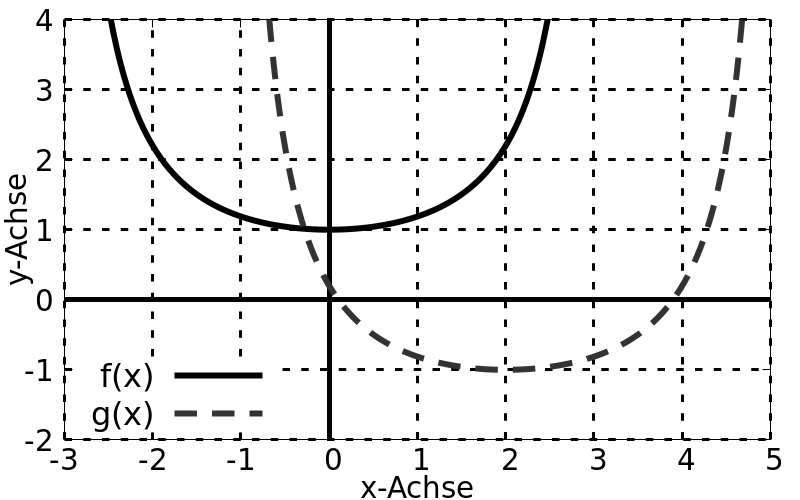
\includegraphics[width=0.95\textwidth]{grid-trial.png}
\end{center}

\begin{enumerate}[label=(\alph*)]
\item (2P) Geben Sie die Koordinaten des Minimums von $f$ und von $g$ an!\\

Minimum von $f$:\\
\bigskip\\
Minimum von $g$:\\
\bigskip
\bigskip

\item (2P) Finden Sie für $g(x)$ eine mögliche Funktionsgleichung!

\bigskip
\bigskip

$g(x)=$

\bigskip
\bigskip
\bigskip

\item (2P) Ermitteln Sie grafisch die Lösungen der Gleichung $\frac{x}{\sin(x)}-2=0$!

\bigskip
\bigskip
\bigskip
\bigskip
\bigskip
\bigskip

\item (1P) Tragen Sie in der Skizze die Taylorentwicklung 1. Grads von $g$ an der Stelle $x_0=2$ ein!

\end {enumerate}

\newpage
\section* {Aufgabe 2}


Ein quadratisches Polynom, welches durch drei paarweise verschiedene Punkte $(x_1,y_1)$, $(x_2,y_2)$ und $(x_3,y_3)$ verläuft, lässt sich wie folgt schreiben:

$$
p_2(x) =
y_1\cdot\frac{x-x_2}{x_1-x_2}\cdot\frac{x-x_3}{x_1-x_3} +
y_2\cdot\frac{x-x_1}{x_2-x_1}\cdot \frac{x-x_3}{x_2-x_3} +
y_3\cdot\frac{x-x_1}{x_3-x_1}\cdot\frac{x-x_2}{x_3-x_2}
$$


\begin{enumerate}[label=(\alph*)]

\item (5P) Finden Sie ein quadratisches Polynom der Form $p_2(x)=ax^2+bx+c$, welches durch die folgenden Punkte verläuft!

\begin{itemize}
\item $(0,1)$
\item $(1,3)$
\item $(2,7)$
\end{itemize}

\bigskip
\bigskip
\bigskip
\bigskip
\bigskip
\bigskip
\bigskip
\bigskip
\bigskip
\bigskip
\bigskip
\bigskip

\item (2P) Beweisen Sie durch Einsetzen, dass für alle Punkte $(x_2,y_2)\in\mathbb{R}^2$ dass Polynom durch diesen Punkt verläuft, d.h. dass $p_2(x_2) = y_2$ gilt!

\end{enumerate}

\newpage
\section* {Aufgabe 3}

Gegeben sei die Funktion $f(x) = x\cdot e^x$ und die Entwicklungsstelle $x_0=0$. Es soll die Taylorentwicklung 2. Grads $p_2(x)$ betrachtet werden.

Taylorformel: $\sum\limits_{n=0}^\infty\frac{f^{(n)}(x_0)}{n!}(x-x_0)^n$

\begin{enumerate}[label=(\alph*)]

\item (4P) Berechnen Sie die Taylorentwicklung 2. Grads von $f$!

\bigskip

$f'(x) = $

\bigskip

$f''(x) = $

\bigskip

$p_2(x) = $

\bigskip
\bigskip
\bigskip
\bigskip
\bigskip

\item (1P) Geben Sie einen Näherungswert für $f(0{,}5)$ an!

\bigskip

$p_2(0{,}5) = $

\bigskip
\bigskip

\item (3P) Die 3. Ableitung lautet $f'''(x)=(x+3)\cdot e^x$. Ermitteln Sie damit eine Abschätzung für den Fehler auf den Wert aus Aufgabe (b)! 

(Hinweis: $\sqrt{e} < \sqrt{4} = 2$)

\bigskip

$|R_2(0{,}5)| \le \frac{|0{,}5-0|^3}{(2+1)!}\cdot\max\limits_{\vartheta\in[0;0{,}5]} f'''(\vartheta) =$

\end{enumerate}

\newpage
\section* {Aufgabe 4}

Gegeben sei die inhomogene DGL

$$2yy' = \frac{x+6}{x^2-4}$$

Durch Termumformung lässt sich zeigen:

$$\frac{x+6}{x^2-4} = \frac{2}{x-2} - \frac{1}{x+2}$$

\begin{enumerate}[label=(\alph*)]

\item (4P) Beweisen Sie die Termumformung mittels Partialbruchzerlegung!

$\frac{x+6}{x^2-4} = $

\bigskip
\bigskip
\bigskip
\bigskip
\bigskip
\bigskip
\bigskip
\bigskip
\bigskip
\bigskip
\bigskip
\bigskip

\item (4P) Ermitteln Sie die allgemeine Lösung der DGL durch Trennung der Variablen!

\bigskip
\bigskip
\bigskip
\bigskip
\bigskip
\bigskip
\bigskip
\bigskip
\bigskip

\end{enumerate}

\newpage
\section*{Zusatzaufgabe (2P)}

Bei der sogenannten Heaviside-Distribution $H$ und der Dirac-Distribution $\delta$ handelt es sich um lineare Funktionale. Diese werden durch ihre Wirkung bei der Integration mit Testfunktionen $\varphi$ definiert:

\begin{itemize}
\item $\int\limits_{-\infty}^\infty \varphi(x) H(x) \d{x} := \int\limits_{0}^\infty \varphi(x) \d{x}$
\item $\int\limits_{-\infty}^\infty \varphi(x) \delta(x) \d{x} := \varphi(0)$
\end{itemize}

Jede Testfunktion $\varphi$ hat unter anderem die Eigenschaft, dass sie außerhalb eines Intervalls um den Ursprung identisch $0$ ist, speziell also auch $\lim\limits_{x\to\pm\infty} \varphi(x) = 0$ gilt.

Zeigen Sie durch partielle Integration, dass die Dirac-Distribution $\delta$ die Ableitung $H'$ der Heaviside-Distribution ist, d.h. dass folgende Beziehung gilt:

\bigskip
 
$\int\limits_{-\infty}^\infty \varphi(x) H'(x) \d{x} = \varphi(0)$

\label{LastTask}

\newpage

\begin{center}
{\bf {\large Musterlösung}}
\end{center}

\begin{center}
{\bf {\large Probeklausur Analysis (3IT19, 3MI19) - 13.02.2020}}
\end{center}

\begin{center}
\textbf{Jeder Anführungspunkt entspricht einem erteilten Bewertungspunkt.} 

Ist ein Rechenschritt falsch, werden für darauf basierende Rechnungen Punkte erteilt (Folgefehler), es sei denn, die Rechnung wird dadurch wesentlich vereinfacht. 
\end{center}

\begin{enumerate}

% Task 1
\item
\begin{enumerate}

\item
\begin{itemize}
\item Minimum von $f$: $(0,1)$ 
\item Minimum von $g$: $(2,-1)$ 
\end{itemize}

\item $g(x) = \frac{x-2}{\sin(x-2)}-2$
\begin{itemize}
\item Für das Verschieben in x-Richtung ($x-2$)
\item Für das Verschieben in y-Richtung ($f(x)-2$)
\end{itemize}

\item Wer genau abliest, kann auch Werte bis zu etwa $\pm 1{,8}$ erhalten.
\begin{itemize}
\item $x_1=-2$
\item $x_2=+2$
\end{itemize}

\item
\begin{itemize}
\item Die horizontale Gerade $y=-1$ wurde eingezeichnet. 
\end{itemize}

\end{enumerate}

% Task 2
\item
\begin{enumerate}

\item
\begin{itemize}
\item $p_2 =
1\cdot\frac{x-1}{0-1}\cdot\frac{x-2}{0-2} +
3\cdot\frac{x-0}{1-0}\cdot \frac{x-2}{1-2} +
7\cdot\frac{x-0}{2-0}\cdot\frac{x-1}{2-1}$
\item $=\frac{1}{2}(x-1)(x-2)-3x(x-2)+\frac{7}{2}x(x-1)$
\item $=\frac{1}{2}(x^2-3x+2)-3(x^2-2x)+\frac{7}{2}(x^2-x)$
\item $=(\frac{1}{2}-3+\frac{7}{2})x^2+(-\frac{3}{2}+6-\frac{7}{2})x+2\cdot\frac{1}{2}$
\item $=x^2+x+1$
\end{itemize}

\item
\begin{itemize}
\item $p_2(x_2) =
y_1\cdot\underbrace{\frac{x_2-x_2}{x_1-x_2}}_0\cdot\frac{x_2-x_3}{x_1-x_3} +
y_2\cdot\underbrace{\frac{x_2-x_1}{x_2-x_1}}_1\cdot\underbrace{\frac{x_2-x_3}{x_2-x_3}}_1 +
y_3\cdot\frac{x_2-x_1}{x_3-x_1}\cdot\underbrace{\frac{x_2-x_2}{x_3-x_2}}_0$
\item $=y_2$
\end{itemize}

\end{enumerate}

% Task 3

\item
\begin{enumerate}

\item
\begin{itemize}
\item $f'(x) = (x+1)e^x$
\item $f''(x) = (x+2)e^x$
\item $f(0) = 0$, $f'(0) = 1$, $f''(0)=2$
\item $p_2(x) \approx 0 + \frac{1}{1!} x + \frac{2}{2!} x^2 = x+x^2$
\end{itemize}

\item
\begin{itemize}
\item $p_2(0{,}5) = 0{,}5+0{,}5^2 = 0{,}75$
\end{itemize}

\item
\begin{itemize}
\item $(x+3)e^x$ ist monoton steigend, Maximum im Intervall $[0;0{,}5]$ ist somit $(0{,}5+3)e^{0{,}5} < 3{,}5\cdot 2 = 7$
\item $|R_2(0{,}5)| \le \frac{0{,}5^3}{6}\cdot 7$
\item $=\frac{7}{48}$
\end{itemize}

\end{enumerate}

% Task 4

\newpage

\item 
\begin{enumerate}

\item
\begin{itemize}
\item $\frac{x+6}{x^2-4} = \frac{A}{x-2}+\frac{B}{x+2}$
\item $\frac{x+6}{x^2-4} = \frac{(A+B)x+(2A-2B)}{(x-2)(x+2)}$
\item $A+B=1$ und $2A-2B=6$
\item $B=-1$ und $A=2$
\end{itemize}

\item 
\begin{itemize}
\item $2y\frac{d{y}}{\d{x}} = \frac{2}{x-2} - \frac{1}{x+2}$
\item $\int 2y \d y = \int \frac{2}{x-2} - \frac{1}{x+2} \d x$
\item $y^2 = 2\ln(|x-2|) - \ln(|x+2|) + C$
\item $y(x) = \pm \sqrt{2\ln(|x-2|) - \ln(|x+2|) + C}$
\end{itemize}

\end{enumerate}

\end{enumerate}

\textbf{Zusatzaufgabe}

\begin{itemize}
\item $\int\limits_{-\infty}^\infty \varphi(x) H'(x) \d{x} = \underbrace{\varphi(x)H(x) \Big|_{-\infty}^\infty}_{\substack{=0\text{, da Testfunktion} \\ \text{im Unendlichen verschwindet}}} - \int\limits_{-\infty}^\infty \varphi'(x)H(x) \d{x}$
\item $ = -\int\limits_0^\infty \varphi'(x) \d{x} = -\varphi(x)\Big|_0^\infty = 0-(-\varphi(0)) = \varphi(0)$
\end{itemize}


\end{document}
